\documentclass[11pt,a4paper]{article}

\usepackage[margin=1.85cm]{geometry}
\usepackage{amsmath,amssymb}
\usepackage{booktabs}
\usepackage{tabularx}
\usepackage{array}
\usepackage{graphicx}
\usepackage{caption}
\usepackage{needspace}
\usepackage[compact]{titlesec}
\usepackage[hidelinks]{hyperref}

\captionsetup{font=small,labelfont=bf,skip=3pt}
\renewcommand{\normalsize}{\fontsize{10.5pt}{12.6pt}\selectfont}
\setlength{\parskip}{2pt}
\setlength{\parindent}{0pt}
\setlength{\emergencystretch}{2em}
\renewcommand{\arraystretch}{1.0}
\setlength{\topsep}{2pt}\setlength{\partopsep}{0pt}
\setlength{\intextsep}{6pt plus 2pt minus 2pt}\setlength{\textfloatsep}{8pt plus 2pt minus 2pt}

\newcommand{\dd}{\,\mathrm{d}}

\title{Delta Hedging of European Options under Model Misspecification:\\
Hedging Error Analysis, Transaction Costs and Empirical Backtesting}
\author{Mehta Prem (2024ADPS0851G)\\
B.E.\ (Hons.) Mathematics and Computing\\
BITS Pilani K K Birla Goa Campus}
\date{MAC F244, Stochastic Calculus and Application to Finance\\
Instructor: Mayank Goel\\
Individual project, 15 November 2026}

\begin{document}
\normalsize
\maketitle
\vspace{-2em}

%--------------------------------------------------------------------
\section{Introduction to the problem}

In the Black--Scholes--Merton (BSM) model a European option can be copied exactly by holding $\Delta(t)$ shares of the stock and adjusting that holding continuously \cite{bs73,merton73,hull}. This is why the option has a unique price, and why a seller who hedges this way carries no risk. Real markets break the model in three ways: we can only trade at discrete times, trading costs money, and the stock does not follow geometric Brownian motion (GBM) with a known, constant volatility.

This project asks how large the hedging error becomes when each of these assumptions is relaxed, and how it behaves statistically. The hedger is the seller of an at-the-money call, and the hedging error is the profit and loss (P\&L) of the hedged position at maturity. We answer four questions:
\begin{enumerate}
  \item \textbf{Discrete rebalancing.} How does the standard deviation of the P\&L shrink as the number of rebalancing dates $n$ grows? Does it follow $\sqrt{\Delta t}$?
  \item \textbf{Wrong volatility.} If the hedger uses a volatility $\sigma_h$ different from the true $\sigma$, what is the P\&L, and does it match the known formula?
  \item \textbf{Wrong dynamics.} If the true stock follows a stochastic-volatility model (Heston) or has jumps (Merton) but the hedger still uses BSM Deltas, how do the bias, variance and tail risk change?
  \item \textbf{Transaction costs.} With proportional costs, which rebalancing frequency minimises the total risk, and does it match Leland's scaling?
\end{enumerate}
We then compare the simulations with a historical delta-hedging backtest on real NIFTY~50 options.

%--------------------------------------------------------------------
\section{Methodology}

\subsection{Mathematical model}

\textbf{Setting.} Let $W(t)$ be a Brownian motion and let the stock follow GBM,
\[
\frac{\mathrm{d}S(t)}{S(t)} = \alpha\dd t + \sigma\dd W(t),\qquad S(t) = S_0\exp\Big\{\sigma W(t) + \big(\alpha - \tfrac12\sigma^2\big)t\Big\},
\]
with constant interest rate $r$, strike $K$, maturity $T$ and $\tau = T-t$. We hedge on a grid $0 = t_0 < \dots < t_n = T$ with steps $\Delta t_i = t_{i+1}-t_i$ and Brownian increments $\Delta W(t_i)\sim N(0,\Delta t_i)$. The quadratic variation $[W,W](T)=T$ gives the rules $(\mathrm{d}W)^2=\mathrm{d}t$, $\mathrm{d}W\,\mathrm{d}t=0$.

\textbf{Replication and the BSM equation.} The seller holds $\Delta(t)$ shares and keeps the rest of the wealth $X(t)$ in the money market, so
\[
\mathrm{d}X = r\big(X - \Delta S\big)\mathrm{d}t + \Delta\,\mathrm{d}S,\qquad \mathrm{d}\big(e^{-rt}X\big) = \Delta\,\mathrm{d}\big(e^{-rt}S\big).
\]
It\^o's formula for $e^{-rt}C(t,S(t))$ gives $e^{-rt}\big[-rC + C_t + \alpha SC_x + \tfrac12\sigma^2S^2C_{xx}\big]\mathrm{d}t + e^{-rt}\sigma SC_x\,\mathrm{d}W$. Asking that $X(t)=C(t,S(t))$ for all $t$, the $\mathrm{d}W$ terms give $\Delta(t)=C_x(t,S(t))$ and the $\mathrm{d}t$ terms give the BSM equation \cite{shreve2}
\[
rC = C_t + rxC_x + \tfrac12\sigma^2x^2C_{xx},\qquad C(T,x)=(x-K)^+ .
\]
The drift $\alpha$ cancels. The solution is $C(t,x)=xN(d_+)-Ke^{-r\tau}N(d_-)$ with $d_\pm(\tau,x)=\frac{1}{\sigma\sqrt\tau}\big[\log\frac{x}{K}+(r\pm\frac{\sigma^2}{2})\tau\big]$, so the delta is $C_x=N(d_+)$ and the gamma is $C_{xx}=N'(d_+)/(x\sigma\sqrt\tau)$.

\textbf{Discrete hedging (Question 1).} Between grid dates the hedge ratio stays at $\Delta(t_i)$. A second-order expansion of $C$, together with the BSM equation, shows that the option and its replicating portfolio differ (up to discounting) by
\[
\tfrac12 C_{xx}\big[(\Delta S)^2 - \sigma^2S^2\Delta t_i\big]\approx \tfrac12 C_{xx}\,\sigma^2S^2\Big[\big(\Delta W(t_i)\big)^2-\Delta t_i\Big]\quad\text{\cite{boyle80,bkl00}}.
\]
This error exists only because $(\Delta W)^2\neq\Delta t$ over a finite step; the rule $(\mathrm{d}W)^2=\mathrm{d}t$ holds only in the limit. It has mean zero, and because $\mathrm{Var}[(\Delta W)^2]=2(\Delta t)^2$ each step contributes variance $\tfrac12(C_{xx}\sigma^2S^2)^2(\Delta t)^2$. Over $T/\Delta t$ steps the total variance is of order $\Delta t$, so the standard deviation scales like $\sqrt{\Delta t}=n^{-1/2}$, and it is largest where the dollar gamma $S^2C_{xx}$ is large: near the strike and near expiry.

\textbf{Wrong volatility (Question 2).} Suppose the seller prices and hedges with $\sigma_h$ (so $C$ solves the BSM equation with $\sigma_h$) while the stock moves with the true $\sigma$. Repeating the steps above, the $\mathrm{d}W$ terms cancel and, using $rC-C_t-rSC_x=\tfrac12\sigma_h^2S^2C_{xx}$, we are left with
\[
\mathrm{d}\Big(e^{-rt}\big(X-C\big)\Big)=\tfrac12\big(\sigma_h^2-\sigma^2\big)e^{-rt}S^2C_{xx}\dd t,
\quad\text{so}\quad
e^{-rT}\,\text{P\&L}=\tfrac12\big(\sigma_h^2-\sigma^2\big)\!\int_0^T\! e^{-rt}S^2C_{xx}\dd t \;\;\text{\cite{elk98}}.
\]
The dollar gamma is positive, so a seller who prices at too high a volatility ($\sigma_h>\sigma$) locks in a gain; the option holder has the opposite sign.

\textbf{Wrong dynamics (Question 3).} In Heston's model \cite{heston93} the variance $V(t)$ follows the CIR process, with $a_V,\beta,\xi$ playing the roles of the CIR constants:
\[
\mathrm{d}S=\alpha S\dd t+\sqrt{V}\,S\dd W_1,\qquad \mathrm{d}V=(a_V-\beta V)\dd t+\xi\sqrt{V}\dd W_2,\qquad \mathrm{d}W_1\mathrm{d}W_2=\rho\dd t .
\]
In the Merton model \cite{merton76} the stock also jumps: $\mathrm{d}S/S=(\alpha-\lambda\bar\kappa)\dd t+\sigma\dd W+(J-1)\dd N$, with $N$ a Poisson process of rate $\lambda$, $\ln J\sim N(m,\delta^2)$ and $\bar\kappa=e^{m+\delta^2/2}-1$. In both models the market is incomplete: variance risk and jump risk cannot be removed with the stock alone, so residual risk remains however often we trade.

\textbf{Transaction costs (Question 4).} With round-trip cost rate $k$, a trade of $q$ shares costs $\tfrac{k}{2}|q|S$. Expected cost grows like $k/\sqrt{\Delta t}$ while risk falls like $\sqrt{\Delta t}$, so an optimal frequency exists. Leland \cite{leland85} shows the expected cost is recovered by pricing and hedging at $\hat\sigma_L^2=\sigma^2\big(1+\sqrt{2/\pi}\,k/(\sigma\sqrt{\Delta t})\big)$.

\subsection{Numerical methodology}

All code is in Python (NumPy, SciPy, pandas), vectorised over 20{,}000 paths with a fixed seed and a test suite. The base case is $S_0=K=100$, $\alpha=r=5\%$, $\sigma=20\%$, $T=1$.
\begin{itemize}
  \item \textbf{Simulation.} GBM and Merton are sampled exactly. For Heston we use full-truncation Euler for the variance \cite{lord10} on a fine grid of 1{,}008 steps, subsampled to the hedging dates, with $\beta=2$, $a_V=0.08$, $V(0)=0.04$. Merton's diffusion variance is reduced so that total variance stays $0.04$; differences from GBM then come from the shape of the distribution, not its level. With 20{,}000 paths the Monte Carlo standard error (bootstrap over the paths) is about 0.7\% of the standard deviation and 1--2\% of the ES (Heston $\xi=0.4$: $1.95\pm0.014$ and $4.86\pm0.066$), but the skewness is only good to $\pm0.04$ to $\pm0.09$ and the excess kurtosis to $\pm0.24$ (Heston) or $\pm1.3$ (Merton), so we do not read small differences in skewness or kurtosis.
  \item \textbf{Hedging engine and risk measures.} The seller receives $C(0,S_0)$, holds $\Delta(t_i)=C_x$ shares, and finances all trades (and costs) in the money market, so P\&L $=X(T)-(S(T)-K)^+$. We report the mean (bias), standard deviation, skewness, kurtosis, and the 5\% value-at-risk and expected shortfall (ES) of the loss.
  \item \textbf{Backtest.} Prices of NIFTY index call options come from the NSE F\&O bhavcopy files for every trading day from January 2015 to November 2026 \cite{nse}, and the NIFTY~50 path from Yahoo Finance \cite{yahoo}. On each date with an NSE expiry exactly 20 trading days ahead, we sell the traded call nearest the money (strike within 1\% of spot) at its listed closing price, hedge it daily ($n=20$) or weekly ($n=4$) at its own \emph{implied} volatility (the $\sigma$ that makes the BSM price equal the market price; $r=6\%$, no dividends), and divide the P\&L by the premium. The \emph{realised} volatility over the option's life is $\hat\sigma=\sqrt{\frac{1}{T_2-T_1}\sum_i[\ln S(t_{i+1})/S(t_i)]^2}$, which estimates $\sigma$ through quadratic variation. The matching simulations use $S_0=K=100$, $\alpha=r=6\%$, $T=20/252$ and $\sigma=14.8\%$, the sample's mean implied volatility, with the premium and Deltas at that $\sigma$; Heston uses the E3 settings ($\beta=2$, $\xi=0.4$, $\rho=-0.7$) with $V(0)=\sigma^2$ (E3 itself uses $\sigma=20\%$, $T=1$). Merton is not simulated here, because the jump parameters of E4 were chosen for one-year options and do not suit a 20-day window. One $\sigma$ is a simplification, because real windows range from calm to crisis; dividing by the premium, which grows roughly in proportion to $\sigma$ for an at-the-money option, puts them on one scale, and the comparison below removes the main regime effect.
\end{itemize}

Code, tests, the notebook and the data notes (\texttt{data/SOURCE.md}) are in the submitted repository, and each experiment script regenerates its tables and figures.

%--------------------------------------------------------------------
\section{Results}

\subsection{Question 1: discrete rebalancing (E1, E6)}

The standard deviation of the P\&L falls from $3.22$ at $n=4$ to $0.218$ at $n=1000$. The log-log slope is $-0.487$ over all $n$ and $-0.500$ for $n\ge52$, matching $\sqrt{\Delta t}$, and the per-step formula predicts the spread within 1\% for $n\ge252$. The mean is about zero at every $n$, so the hedge is unbiased under the true model. The error follows the dollar gamma: with weekly hedging it peaks near $K=110$ ($1.02$, against $0.47$ at $K=80$).

\subsection{Question 2: wrong volatility (E2)}

\Needspace{7\baselineskip}
The simulated mean P\&L of the seller agrees with the formula to within about one standard error:

\begin{center}\small
\begin{tabular}{lccccc}
\toprule
$\sigma_h/\sigma$ & 0.50 & 0.75 & 1.00 & 1.25 & 1.50 \\
\midrule
simulated mean & $-3.818$ & $-1.947$ & $0.002$ & $1.979$ & $3.967$ \\
formula        & $-3.823$ & $-1.949$ & $0.000$ & $1.978$ & $3.966$ \\
\bottomrule
\end{tabular}
\end{center}

A 25\% volatility error moves the mean P\&L by about 2 on a premium of $10.45$, far more than the discretisation error at $n=1000$ ($0.22$).

\begin{figure}[ht]
  \centering
  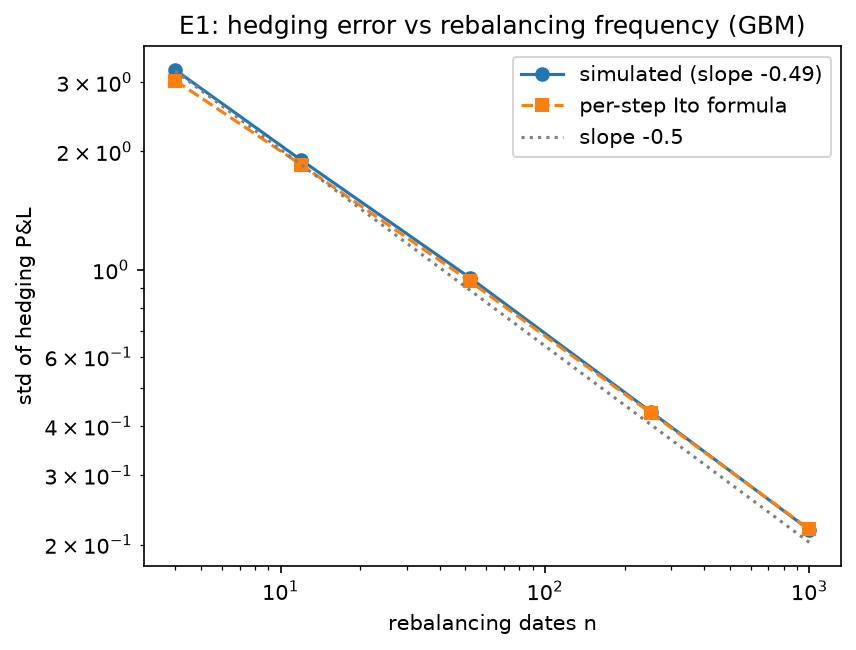
\includegraphics[width=0.40\linewidth]{../results/figures/e1_rebalancing.png}\hfill
  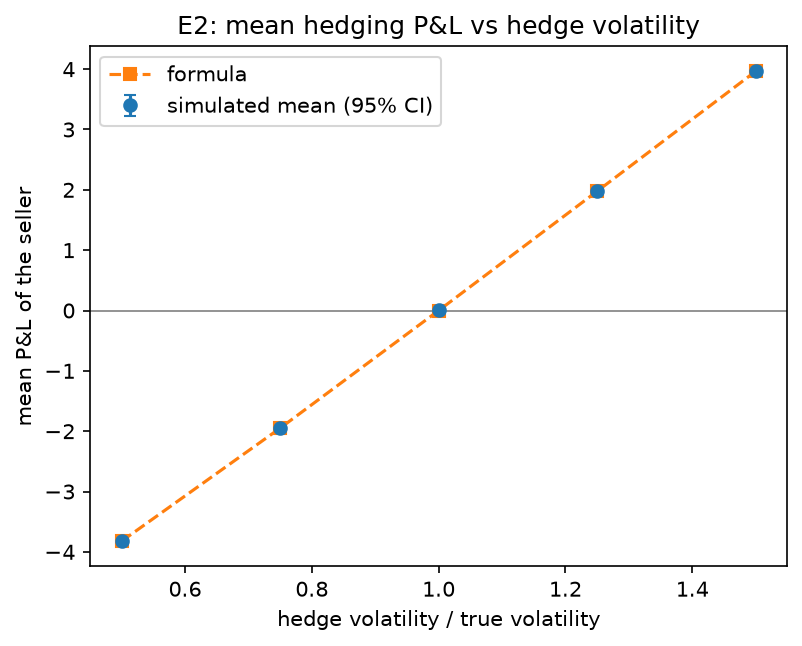
\includegraphics[width=0.40\linewidth]{../results/figures/e2_mean_pnl.png}
  \caption{Left, E1: standard deviation of the P\&L against $n$ (log-log), with the per-step formula and the $-1/2$ slope. Right, E2: simulated mean P\&L of the seller (95\% interval) against the formula.}
  \label{fig:e1e2}
\end{figure}

\Needspace{9\baselineskip}
\subsection{Question 3: wrong dynamics (E3, E4)}

Daily hedging ($n=252$), all rows at the same $n$:

\begin{center}\small
\begin{tabular}{lccccc}
\toprule
model & mean & std & skew & excess kurtosis & 5\% ES \\
\midrule
GBM                                  & $0.002$ & $0.43$ & $-0.15$ & $1.9$  & $0.99$ \\
Heston $\xi=0.4,\ \rho=-0.7$          & $0.157$ & $1.95$ & $-0.93$ & $2.1$  & $4.86$ \\
Heston $\xi=0.6,\ \rho=-0.7$          & $0.453$ & $2.65$ & $-1.28$ & $3.2$  & $6.70$ \\
Merton $\lambda=0.5,\ m=-0.1$         & $0.106$ & $2.18$ & $-3.29$ & $15.3$ & $7.38$ \\
\bottomrule
\end{tabular}
\end{center}

Risk grows with the vol-of-vol and with the size and frequency of jumps, and it does not vanish as $n$ grows: for Heston ($\xi=0.4$) the standard deviation only drops from $2.83$ at $n=12$ to $1.91$ at $n=1008$, and for Merton it stops at $2.18$, while GBM falls to $0.22$. Correlation matters too: at $\xi=0.4$ the standard deviation is $1.48$ for $\rho=-0.9$ but $2.55$ for $\rho=0$, because strongly correlated variance shocks are partly hedged by the stock. Under jumps the short-gamma seller loses on big moves either way, giving the long left tail.

\subsection{Question 4: transaction costs (E5)}

The simulated cost matches Leland's formula within 2\%, and pricing at $\hat\sigma_L$ removes the cost bias. Minimising the root-mean-square error (RMSE) of the net P\&L over the grid of $n$ values 12, 26, 52, 78, 104, 156, 208, 252, 378, 504, 756 and 1000 gives $n^*=378,156,78,26$ for $k=0.001,0.0025,0.005,0.01$. The closed form $n^*=s/a$ gives $398,159,80,40$, so $n^*$ falls roughly like $1/k$ for small $k$; at $k=0.01$ the grid is coarse and the RMSE is flat near its minimum, and from $k=0.005$ to $0.01$ the simulated $n^*$ falls by a factor of 3, not 2. The optimum also depends on our choice of RMSE as the criterion.


\subsection{Comparison with real data: NIFTY 50 options (E7)}

\Needspace{10\baselineskip}
We obtain 372 windows between January 2015 and October 2026 (monthly expiries before 2019, weekly after; median premium 353 index points). P\&L divided by the premium:

\begin{center}\small
\begin{tabular}{lccccc}
\toprule
sample & mean & std & skew & excess kurtosis & 5\% ES \\
\midrule
listed options, daily hedging   & $0.058$ & $0.247$ & $-1.10$ & $2.5$  & $0.63$ \\
listed options, weekly hedging  & $0.008$ & $0.398$ & $-1.57$ & $5.8$  & $1.10$ \\
GBM, daily                      & $0.001$ & $0.167$ & $-0.37$ & $1.7$  & $0.39$ \\
Heston, daily                   & $0.007$ & $0.226$ & $-0.84$ & $2.8$  & $0.57$ \\
\bottomrule
\end{tabular}
\end{center}

\begin{figure}[ht]
  \centering
  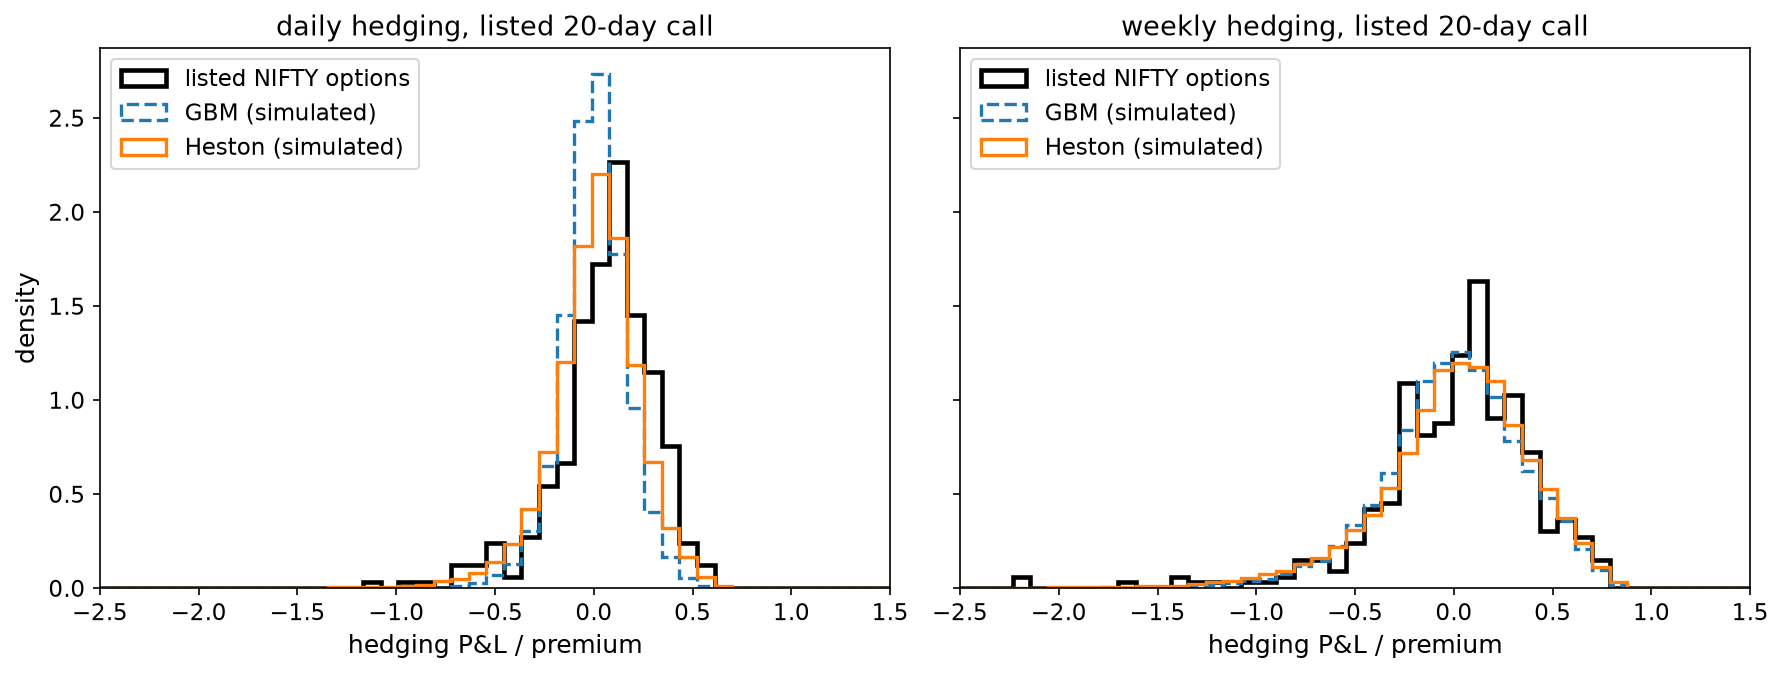
\includegraphics[width=0.8\linewidth]{../results/figures/e7_distribution.png}
  \caption{E7: P\&L / premium of the listed-option backtest against the simulated models.}
  \label{fig:e7}
\end{figure}

\textbf{Why the mean is positive.} Listed implied volatility averaged $14.8\%$, while NIFTY actually realised $13.5\%$, and implied was higher in 68\% of windows. A seller who charges for $14.8\%$ but faces $13.5\%$ gains, exactly as in the wrong-volatility result of E2. Applying the E2 formula window by window, with the realised volatility as $\sigma$ and the implied volatility as $\sigma_h$, gives an average of $23.0$ index points against $23.6$ observed, with correlation $0.87$.

\textbf{Is the extra spread a stochastic-volatility effect?} The raw P\&L is clearly larger and more skewed than GBM: for daily hedging the standard deviation is $0.247$ (95\% bootstrap interval $0.213$ to $0.280$) against $0.167$ for GBM, and the skewness is $-1.10$ ($-1.47$ to $-0.66$) against $-0.37$. This comparison is not like for like, however. Each real window is hedged at its own implied volatility, so windows differ in the gap between implied and realised volatility, and by E2 this adds spread and skew; the simulations hedge at the true $\sigma$ and have no such term. To remove it we use the exact version of the wrong-volatility formula, which weights each day's squared return by that day's dollar gamma:
\[
\text{P\&L}\approx\tfrac12\sum_i e^{r(T-t_i)}\,S(t_i)^2C_{xx}(t_i,S(t_i))\Big[\sigma_h^2\Delta t_i-\Big(\ln\tfrac{S(t_{i+1})}{S(t_i)}\Big)^2\Big].
\]
The window-average $\hat\sigma$ used above is accurate only if the variance is spread evenly over the window. The entry of 26 February 2020 shows why it is not: the index crashed while the option was far out of the money, so its gamma was close to zero on the crash days and they cost little, yet the window-average formula predicts a loss of $3.6$ times the premium against an actual $0.44$. The gamma-weighted formula predicts $0.56$, and over all windows it raises the correlation with the real daily P\&L from $0.87$ to $0.95$ (average $23.7$ against $23.6$ index points observed). The table below applies it to the real windows and to the simulated paths.

\begin{center}\small
\begin{tabular}{lcc}
\toprule
\multicolumn{3}{c}{standard deviation of (P\&L $-$ formula) / premium} \\
\midrule
sample & daily & weekly \\
\midrule
listed, all windows (372)              & $0.090$ & $0.222$ \\
listed, no daily move above 4\% (355)  & $0.041$ & $0.117$ \\
listed, a daily move above 4\% (17)    & $0.374$ & $0.889$ \\
GBM (simulated)                        & $0.041$ & $0.118$ \\
Heston (simulated)                     & $0.051$ & $0.141$ \\
\bottomrule
\end{tabular}
\end{center}

What is left is the higher-order error of a second-order formula, and it comes from large single-day moves. Without a daily move above 4\% (a threshold we chose; daily moves that large are 0.6\% of all days) the real residual is as small as GBM's, and the 17 windows with such a move have residuals about ten times larger. The result is similar for thresholds of 3\% and 5\% ($0.039$ and $0.061$ daily). Because the formula uses each path's own squared returns, it absorbs any volatility clustering and cannot separate Heston from GBM. So the real hedging error is larger and more skewed than GBM. A stochastic-volatility effect is consistent with this, but variation of volatility across windows also contributes, and the gamma-weighted wrong-volatility effect explains most of it; the rest comes from a few large daily moves.

%--------------------------------------------------------------------
\section{Conclusions}

\begin{center}
\small
\begin{tabularx}{\linewidth}{>{\raggedright\arraybackslash}p{2.4cm} >{\raggedright\arraybackslash}X >{\raggedright\arraybackslash}X}
\toprule
Question & Answer & Evidence \\
\midrule
1.\ Discrete rebalancing &
Yes. The error is unbiased and its standard deviation scales like $\sqrt{\Delta t}=n^{-1/2}$, because $\mathrm{Var}[(\Delta W)^2]=2(\Delta t)^2$. &
Slope $-0.50$; formula within 1\% (E1, E6) \\
2.\ Wrong volatility &
Yes. The seller's discounted P\&L is $\tfrac12(\sigma_h^2-\sigma^2)\int_0^T e^{-rt}S^2C_{xx}\dd t$. &
Simulated means match to about one standard error (E2) \\
3.\ Wrong dynamics &
Bias, variance and tail risk all grow, and the residual does not vanish with more frequent hedging, because the market is incomplete. &
At $n=252$: Heston ($\xi=0.4$) std $1.95$ against $0.43$ for GBM, ES $4.86$ against $0.99$; Merton std $2.18$, ES $7.38$ (E3, E4) \\
4.\ Transaction costs &
An interior optimal frequency exists; the cost matches Leland, and under RMSE $n^*$ falls roughly like $1/k$ for small $k$. &
$n^*=378,156,78,26$ on a grid of 12 values from 12 to 1000; cost within 2\% (E5) \\
Real data &
Larger and more skewed than GBM, mostly through the gamma-weighted wrong-volatility effect; the rest comes from a few large daily moves, and Heston and GBM cannot be separated. &
372 windows; gamma-weighted formula correlation $0.95$; residual std $0.041$ without large moves, as for GBM (E7) \\
\bottomrule
\end{tabularx}
\end{center}

\textbf{Limitations.} Prices are end-of-day closes, and older NSE files give no underlying price, so we keep strikes within 1\% of the NIFTY close. There are about 130 independent windows, only four of them from the 2020 crash, and the data cannot separate Heston from GBM. The rate is a constant 6\% and dividends are ignored. The Heston and Merton parameters are illustrative, not calibrated, and the optimal $n$ depends on the RMSE criterion.

%--------------------------------------------------------------------
\begin{thebibliography}{99}\scriptsize
\setlength{\itemsep}{0pt}\setlength{\parskip}{0pt}

\bibitem{bs73} Black, F.\ and Scholes, M.\ (1973). The pricing of options and corporate liabilities. \emph{Journal of Political Economy}, 81(3), 637--654.

\bibitem{merton73} Merton, R.C.\ (1973). Theory of rational option pricing. \emph{Bell Journal of Economics and Management Science}, 4(1), 141--183.

\bibitem{hull} Hull, J.C.\ (2009). \emph{Options, Futures, and Other Derivatives}, 7th edition. Prentice-Hall.

\bibitem{shreve2} Shreve, S.E.\ (2004). \emph{Stochastic Calculus for Finance II: Continuous-Time Models}. Springer.

\bibitem{boyle80} Boyle, P.P.\ and Emanuel, D.\ (1980). Discretely adjusted option hedges. \emph{Journal of Financial Economics}, 8(3), 259--282.

\bibitem{bkl00} Bertsimas, D., Kogan, L.\ and Lo, A.W.\ (2000). When is time continuous? \emph{Journal of Financial Economics}, 55(2), 173--204.

\bibitem{elk98} El Karoui, N., Jeanblanc-Picqu\'e, M.\ and Shreve, S.E.\ (1998). Robustness of the Black and Scholes formula. \emph{Mathematical Finance}, 8(2), 93--126.

\bibitem{heston93} Heston, S.L.\ (1993). A closed-form solution for options with stochastic volatility with applications to bond and currency options. \emph{Review of Financial Studies}, 6(2), 327--343.

\bibitem{merton76} Merton, R.C.\ (1976). Option pricing when underlying stock returns are discontinuous. \emph{Journal of Financial Economics}, 3(1--2), 125--144.

\bibitem{leland85} Leland, H.E.\ (1985). Option pricing and replication with transactions costs. \emph{Journal of Finance}, 40(5), 1283--1301.

\bibitem{lord10} Lord, R., Koekkoek, R.\ and van Dijk, D.\ (2010). A comparison of biased simulation schemes for stochastic volatility models. \emph{Quantitative Finance}, 10(2), 177--194.

\bibitem{nse} National Stock Exchange of India. F\&O bhavcopy files, NIFTY index options, 2015--2026, \url{https://nsearchives.nseindia.com/}. Downloaded 15 November 2026.

\bibitem{yahoo} Yahoo Finance. NIFTY~50 (\^{}NSEI) daily closes, retrieved with the \texttt{yfinance} Python library (v1.8.0) on 15 November 2026.

\end{thebibliography}

\end{document}
